\newpage

\anonchapter{Лабораторная работа №4}
\setcounter{chapter}{4}

\begin{center}
Определение времени жизни неосновных носителей заряда по спаду фотопроводимости\\
(4 часа)
\end{center}

\section{Цель работы}
Определение рекомбинационного времени жизни в непрямозонных полупроводниках по спаду фотопроводимости бесконтактным СВЧ методом.

\section{Теоретическая часть}

\subsection{Генерация и рекомбинация}
При освещении полупроводника светом с энергией, превышающей ширину запрещённой зоны, или при протекании тока через неоднородный полупроводник, в нём могут появляться неравновесные или избыточные носители заряда. По аналогии с равновесной концентрацией носителей, имеющей место в стационарном состоянии, концентрация в данном случае носит название неравновесной. Её можно записать как:

\begin{equation}
n = n_{0} + \Delta n
\end{equation}
где $n_{0}$ - равновесная концентрация, $\Delta n$ - концентрация избыточных носителей заряда.

Изменение концентрации под освещением называется оптической генерацией. Если концентрация избыточных носителей мала по сравнению с равновесной, говорят о низком уровне генерации (или низком уровне инжекции, если речь идёт об инжекции носителей из контакта). Уровень генерации можно расчитать по закону Бугера-Ламберта. Для света интенсивности $I$ и образца с толщиной, превышающей величину $\frac{1}{\alpha}$, где $\alpha$ - коэффициент поглощения света, можно записать:

\begin{equation}
G(x) = -\frac{d I(x)}{d x} = \alpha I(x) = I_{0} (1-R) \exp(-\alpha x)
\end{equation}
где $R$ - коэффициент отражения.

Для тонких образцов стоит учитывать многократное отражение:

\begin{equation}
G(x) = I_{0} \frac{1-R}{1-R^{2} \exp(-2 \alpha d)} \exp(-\alpha x)
\end{equation}

Процесс исчезновения пары избыточных носителей при взаимодействии называется рекомбинацией.

Рекомбинация в объёме полупроводника может протекать по трём основным механизмам.

\begin{enumerate}
\item Межзонная рекомбинация - это переход электронов из зоны проводимости в валентную зону. Такой переход сопровождается испусканием энергии, которая в прямозонных полупроводниках излучается в виде света. Поэтому такую рекомбинацию называют излучательной. В непрямозонных материалах, таких как кремний и германий, излучательная рекомбинация не наблюдается, а коэффициент межзонной рекомбинации очень мал.
\item Рекомбинация через локальные центры или рекомбинация Шоккли-Рида-Холла - это процесс, при котором электроны переходят из зоны проводимости на разрешённые уровни в запрещённой зоне (их роль обычно играют атомы примеси и дефекты решётки), а уже с них - в валентную зону.
\item Оже-рекомбинация - это процесс, при котором электрон, переходя в валентную зону, отдаёт часть своей энергии другому электрону в зоне проводимости, благодаря чему тот переходит на более высокий уровень внутри зоны.
\end{enumerate}

Для монокристаллического кремния доминирующим механизмом является рекомбинация Шоккли-Рида-Холла.

Рассмотрим полупроводник n-типа. При низком уровне инжекции один и тот же примесный центр будет либо заполнен электронами (в электронном материале, либо дырками (в дырочном материале). Тогда при рекомбинации пары в n–типе сначала должна быть захвачена дырка из валентной зоны (электрон с центра уходит в валентную зону), затем на это место захватывается электрон из зоны проводимости. Время жизни определяется скоростью захвата дырки на примесный центр, то есть, временем жизни дырки. Поэтому в случае малого уровня инжекции говорят о времени жизни неосновных носителей заряда, хотя оно по-прежнему характеризует время жизни избыточной электронно-дырочной пары.

Скорость генерации и рекомбинации носителей характеризуется приращением концентрации в единицу времени. Процесс изменения концентрации со временем описывается уравнением непрерывности:
\begin{equation}
\frac{\partial n}{\partial t} = G_{n} - R_{n} + \frac{1}{e} \operatorname{div} j
\end{equation}

В стационарном состоянии при отсутствии градиента концентрации тепловая генерация и рекомбинация полностью уравновешивают друг друга: $G_{0} = R_{0}$. В то же время изменение внешних условий приводит к изменению уровня генерации: $G = G_{0} + \Delta G$. При этом изменяется концентрация избыточных носителей $n = n_{0} + \Delta n$. Рекомбинация, как в равновесном, так и в неравновесном случае характеризуется одинаковой величиной $\omega$, равной вероятности рекомбинации одного носителя за единицу времени. Полное число носителей, прорекомбинировавших за единицу времени, таким образом, составит $R = \omega n$. Вероятность имеет размерность обратного времени, поэтому можно ввести характерную величину, называемую временем жизни $\tau = \frac{1}{\omega}$. Тогда

\begin{equation}
\frac{\partial n}{\partial t} = G_{n} - R_{n} = G_{0} + \Delta G - \frac{n_{0} + \Delta n}{\tau} = \Delta G - \frac{\Delta n}{\tau}
\label{eq4_contin}
\end{equation}

Если величина $\tau$ не зависит от концентрации носителей, то есть, не меняется со временем, то она численно равно времени, за которое избыточная концентрация неравновесных носителей спадает в $e$ раз ($e = 2.72$):

\begin{equation}
\Delta n(t) = \Delta n_{0} \exp \left( -\frac{t}{\tau} \right)
\end{equation}
что является точным решением дифференциального уравнения (\ref{eq4_contin}) при условии $\Delta G = 0$.

В общем случае $\tau$ может зависеть от величины избыточной концентрации или уровня инжекции. В таком случае из (\ref{eq4_contin}) выводится понятие мгновенного времени жизни, которое есть отношение избыточной концентрации неравновесных носителей к скорости изменения этой концентрации из-за рекомбинации в объёме:

\begin{equation}
\tau = -\frac{\Delta n}{\partial n / \partial t}
\end{equation}

В одном образце рекомбинация может протекать через различные механизмы, каждый из которых характеризуется своей вероятностью $\omega_{i}$. В таком случае общая вероятность рекомбинации одной частицы равна сумме вероятностей для каждого механизма:

\begin{equation}
\omega = \sum\limits_{i} {\omega_{i}} \rightarrow \frac{1}{\tau} = \sum\limits_{i} {\frac{1}{\tau_{i}}}
\end{equation}

Если $\tau$ не зависит от концентрации, его можно определить по спаду фотопроводимости, то есть, по изменению со временем добавочной части электропроводности, возникающей при облучении образца светом. Стандарт ГОСТ рекомендует для этого определять время, за которое избыточная фотопроводимость спадает в $e$ раз после выключения освещения. Также существуют стационарные методы измерения времени жизни, в которых $\tau$ моно определить по абсолютной величине фотопроводимости, если известна скорость генерации: $\tau = \frac{\Delta \sigma_{max}}{e G \mu}$.

\subsection{Скорость поверхностной рекомбинации и эффективное время жизни}

В идеальном случае сигнал релаксации неравновесной концентрации носителей заряда описывается экспоненциальной функцией с параметром $\tau$. Однако образцы для измерения имеют конечные размеры. Через поверхностные состояния идут дополнительные к объемным процессы рекомбинации, что уменьшает величину измеряемого или эффективного времени жизни $\tau_{eff}$ и искажает форму релаксационной кривой. Рекомбинация на поверхности характеризуется скоростью поверхностной рекомбинации $S$, которая зависит от обработки поверхности. Для пассивированных пластин монокристаллического кремния эта скорость не превышает десятков см/с, для шлифованных образцов может превышать десятки тысяч см/с. Учёт поверхностной рекомбинации позволяет записать граничные условия для образца толщиной $2 a$ как:

\begin{equation}
D_{p} \frac{\partial n}{\partial x} = \pm s \Delta n
\end{equation}

Для описания релаксационной кривой необходимо решать уравнение непрерывности (\ref{eq4_contin}) при отсутствии генерации в объёме, но с учётом потока зарядов. Пусть пластина имеет n-тип проводимости. Будем считать, что центры прилипания отсутствуют, а уровень генерации низкий. Избыточные носители созданы импульсом света. Тогда уравнение непрерывности в одномерном случае будет иметь вид:

\begin{equation}
\frac{\partial n}{\partial t} = -\frac{\Delta n}{\tau} + \mu_{p} E \frac{\partial n}{\partial x} + D_{p} \frac{\partial^2 n}{\partial x^2}
\label{eq4_relaxation}
\end{equation}
где $D_{p}$ - коэффициент диффузии дырок, $E$ - поле, возникающее из-за градиента заряда.

Считая внутреннее поле $E$ малым, решение уравнения (\ref{eq4_relaxation}) можно записать как

\begin{equation}
\Delta n(x,t) = G \cos(A x) \exp \left( -t \left[ \frac{1}{\tau_{p}} + D_{p} \frac{\xi^2}{a^2} \right] \right)
\end{equation}
где $\xi$ - корень трансцендентного уравнения $\frac{D_{p}}{a S} \xi = \ctg \xi$.

Трансцендентное уравнение, определяющее $\xi$ имеет первое решение в интервале $\left( 0, \frac{\pi}{2} \right)$, второе решение - в интервале $\left( \pi, \frac{3 \pi}{2} \right)$ и т.д. При этом существует два точных решения этого уравнения в области $\left( 0, \frac{\pi}{2} \right)$, расположенных в крайних точках. Если $S \rightarrow 0$ то $\xi_{1} \rightarrow 0$, а если $S \rightarrow \infty$ то $\xi_{1} \rightarrow \frac{\pi}{2}$. Первый случай реализуется при измерении тонких (менее 100 мкм) пластин. В этом случае

\begin{equation}
\frac{1}{\tau_{eff}} = \frac{1}{\tau} + \frac{2 S}{d}
\end{equation}

Второй случай реализуется в образцах с непассивированной поверхностью

\begin{equation}
\frac{1}{\tau_{eff}} = \frac{1}{\tau} + \frac{\pi^2 D}{d^2}
\end{equation}

В общем случае для расчёта времени жизни можно использовать сумму этих двух решений:

\begin{equation}
\frac{1}{\tau_{eff}} = \frac{1}{\tau} + \frac{1}{\frac{d^2}{\pi^2 D} + \frac{d}{2 S}}
\label{eq4_pavelka}
\end{equation}

\section{Методика измерения и описание установки}

Работа происходит в два этапа. На первом измеряется эффективное время жизни на установке, реализующей бесконтактный СВЧ метод. На втором проводится моделирование релаксационной кривой для определения скорости поверхностной рекомбинации.

\subsection{Работа с лабораторной установкой}

Схема установки для измерения времени жизни бесконтактным СВЧ методом по спаду фотопроводимости приведена на рисунке \ref{pic4_taumetr}.

\begin{figure}[h!]\centering
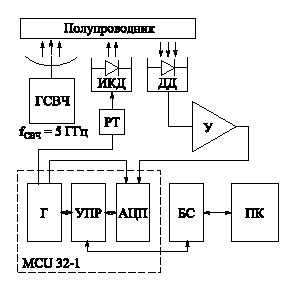
\includegraphics[height=6cm]{pic4_taumetr.eps}
\caption{Схема установки}
\label{pic4_taumetr}
\end{figure}

Генератор СВЧ излучения ГСВЧ создаёт в волноводе стоячую волну. Частота излучения 2.5 ГГц. Через кольцевой зазор в волноводе часть излучения выходит наружу и поглощается в полупроводнике. Величина поглощённой СВЧ мощности пропорциональна концентрации свободных носителей заряда. Данные об интенсивности СВЧ излучения снимаются детекторным СВЧ диодом ДД, усиливаются и отправляются в микроконтроллер.

При освещении полупроводника монохроматическим светом при помощи инфракрасного светодиода ИКД концентрация свободных носителей увеличивается. Длина волны светодиода 1.06 мкм. Прибор снимает изменение концентрации и выводит результат на экран компьютера. Длительность импульса задаётся программно. Запуск измерения производится кнопкой <<Измерить>>, файл с результатами сохраняется в памяти устройства.

Зная, что концентрация избыточных носителей изменяется по закону $\delta n(t) = \Delta n_{0} \exp(-\frac{t}{\tau})$, постоянную $\tau$ можно получить, построив график зависимости $\ln n(t)$. Котангенс угла наклона такого графика будет равен времени жизни.

Влияние поверхностной рекомбинации приводит к искажениям релаксационной кривой в начальной области. Стандарт SEMI MF-1535 рекомендует измерять время жизни по участку от 45\% до 5\% от максимального уровня выходного сигнала. Предел 5\% ограничивает уровень шума.

\subsection{Работа с программой моделирования релаксационной кривой}

Постоянная спада фотопроводимости зависит не только от свойств материала, из которого сделан образец, но и от состояния поверхности. В первом приближении формула (\ref{eq4_pavelka}) даёт близкую оценку величины рекомбинационного времени жизни в объёме полупроводника и скорости поверхностной рекомбинации. Для более точного анализа численными методами решается уравнение непрерывности. Программа расчитывает время жизни в объёме, исходя из данных о концентрации центров рекомбинации, затем строит профиль статического распределения носителей при данном уровне освещения. Затем рассчитывает скорость изменения электропроводности, анализируя изменение концентрации при рекомбинации носителей. После этого расчитывает время жизни по контангенсу угла наклона логарифма кривой спада фотопроводимости и выводит на экран полученное значение эффективного времени жизни с учётом рекомбинации на поверхности. Данные о скорости поверхностной рекомбинации, толщине образца, типе проводимости, концентрации глубоких центров и длине волны засвечивающего светодиода вводятся вручную.

В ходе работы требуется построить зависимость измеряемого времени жизни $\tau_{eff}$ от времени жизни в объёме $\tau$. Для этого на каждом шаге подбирается такая концентрация глубоких уровней $N_{t}$, чтобы $\tau$ менялось от одной микросекунды до 16 миллисекунд, увеличиваясь в два раза на каждом шаге.

\section{Порядок проведения работы и указания по технике безопасности}

\begin{enumerate}
\item Включить компьютер и установку АПК <<Тауметр>>, запустить программу для измерения времени жизни неравновесных носителей заряда.
\item Поместить образец на предметный стол установки, так чтобы образец полностью закрывал кольцевой зазор.
\item Выбрать шаг по времени так, чтобы чтобы релаксационная кривая к концу измерения интервала выходила на насыщение. Время измерения составляет 1000 шагов. Для уменьшения погрешностей проводят серию измерений с одинаковыми параметрами.
\item Выбрать ток засветки так, чтобы уровень инжекции оставался низким. Для этого сравниваются результаты измерения при разных токах лазера, и если значения отличаются более чем на 30\%, ток необходимо уменьшить по меньшей мере вдвое.
\item Расчет эффективного времени жизни производится автоматически. Нулевая точка выбирается как среднее значение последних десяти измерений, максимальная – через два шага после выключения подсветки. В окне «ГОСТ» появляется значение времени, равное моменту времени, в который максимальное значение сигнала уменьшается в 2,7 раз. В окне «ASTM» появляется значение котангенса угла наклона логарифма релаксационной кривой на участке от 45 до 5\% первоначальной интенсивности.
\item Записать результаты измерения в файл для последующей обработки.
\item Запустить программу для расчёта времени жизни.
\item Ввести толщину образца, тип проводимости, длин волны засвечивающего лазера. Сделать предположение о концентрации глубоких уровней $N_{t}$ (величина, обратно пропорциональная времени жизни в объёме полупроводника).
\item Ввести скорость поверхностной рекомбинации, исходя из предположений о пассивации образца.
\item Рассчитать профиль статического распределения, затем запустить расчёт спада фотопроводимости и расчёт времени жизни (ASTM).
\item Результаты внести в таблицу \ref{table4}.
\end{enumerate}

Электрический ток в схеме не превышает 300 мА. При выполении работы действует стандартная техника безопасности при работе с компьютером.

\begin{table}[h!]
\caption{Измерение магнетосопротивления}
\begin{center}
\begin{tabular}{c|c|c}
№ & $\tau$ & $\tau_{eff}$ \\
\hline
& мкс & мкс \\
\hline
\end{tabular}
\end{center}
\label{table4}
\end{table}

\section{Обработка результатов эксперимента}

\begin{enumerate}
\item Из результатов измерения выделить кривую спада фотопроводимости, построить зависимость логарифма избыточной концентрации от времени, выделить линейный участок графика.
\item Меняя концентрацию глубокой примеси в образце при моделировании, построить график зависимости эффективного времени жизни от времени жизни в объёме образца для данной толщины.
\item По полученным данным определить величину времени жизни в объёме полупроводника.
\item Определить погрешность измерения времени жизни неравновесных носителей заряда.
\item Сравнить результаты измерения с формулой (\ref{eq4_pavelka}). Сделать выводы о применимости формулы для образцов данной толщины.
\end{enumerate}

\section{Контрольные вопросы}

\begin{enumerate}
\item Определение времени жизни неравновесных носителей заряда и диффузионной длины неравновесных носителей заряда.
\item Зависимость времени жизни и диффузионной длины неосновных носителей заряда от параметров материала.
\item Центры рекомбинации и прилипания неравновесных носителей заряда.
\item Диффузия и дрейф носителей в полупроводнике.
\item Нестационарные методы измерения времени жизни.
\item Влияние поверхностной рекомбинации на время жизни неравновесных носителей заряда.
\item Соотношение Эйнштейна для определения коэффициента диффузии свободных носителей заряда.
\item Влияние центров прилипания на результаты измерения времени жизни неравновесных носителей заряда.
\item Основные механизмы рекомбинации в полупроводниках.
\item Основные механизмы генерации в полупроводниках.
\end{enumerate}

\section{Литература}
\begin{enumerate}
\item В.В. Батавин, Ю.А. Концевой, Ю.В. Федорович. Измерение параметров полупроводниковых материалов и структур. М.: Радио и связь, 1985 г.
\item Л.П. Павлов. Методы определения основных параметров полупроводниковых материалов. М.: Высшая школа, 1975 г.
\item Шалимова К.В. Физика полупроводников. СПб.: Лань 2011.
\end{enumerate}